\documentclass[10pt]{article}
\usepackage{graphicx}
\usepackage[margin=1.5cm]{geometry}
\usepackage{amsmath}
\def\brcurs{{\mbox{$\resizebox{.16in}{.08in}{
\includegraphics{BoldR}}$}}}
\def\rcurs{{\mbox{$\resizebox{.16in}{.08in}{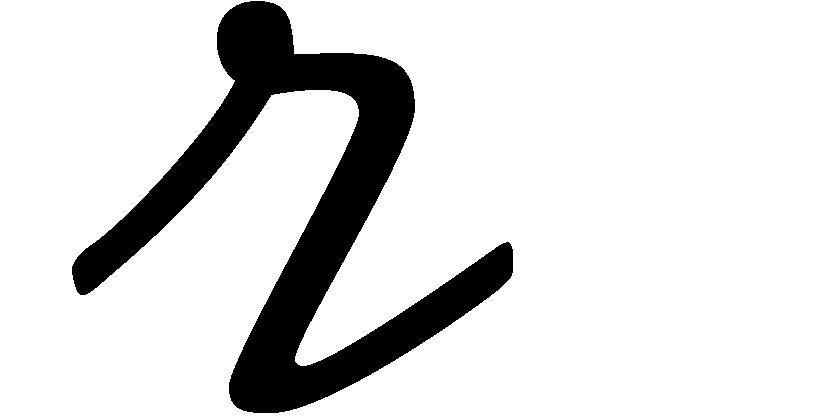
\includegraphics{ScriptR}}$}}}

\begin{document}
\twocolumn

\title{Tuesday Warm-up: Biot-Savart and Amp\`{e}re's Laws}
\author{Prof. Jordan C. Hanson}

\maketitle

\section{Memory Bank}

\begin{itemize}
\item \textbf{The Biot-Savart Law}, for steady currents:
\begin{equation}
\mathbf{B}(\mathbf{r}) = \frac{\mu_0 I}{4\pi}\int \frac{d\mathbf{l}'\times \hat{\brcurs}}{\rcurs^2}
\end{equation}
\item \textbf{Amp\`{e}re's Law}, differential form:
\begin{equation}
\nabla \times \mathbf{B} = \mu_0 \mathbf{J}
\end{equation}
\item \textbf{Amp\`{e}re's Law}, integral form:
\begin{equation}
\oint \mathbf{B} \cdot d\mathbf{l} = \mu_0 I_{\rm enc}
\end{equation}
\end{itemize}

\begin{figure}
\centering
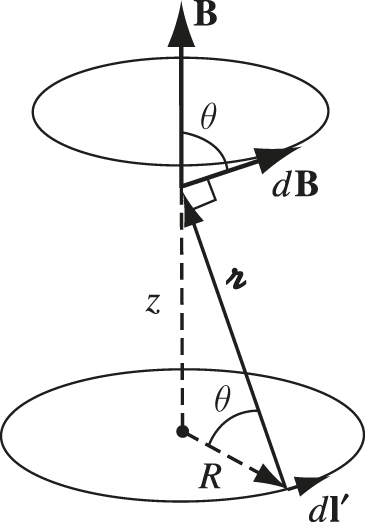
\includegraphics[width=0.15\textwidth]{figures/5_20.jpg} \hspace{0.5cm}
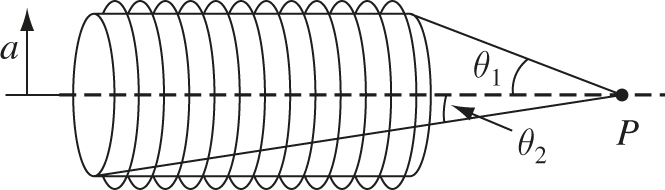
\includegraphics[width=0.3\textwidth]{figures/5_24.jpg}
\caption{\label{fig:1} (Left) The $\mathbf{B}$-field above a circular loop of current. (Right) A solenoid.}
\end{figure}

\section{Biot-Savart Law}

\begin{enumerate}
\item Consider Fig. \ref{fig:1} (left). Find the magnetic field a distance $z$ above the center of a circular loop of radius $R$, which carries a steady current $I$. \\ \vspace{5cm}
\item Consider Fig. \ref{fig:1} (right).  Find the magnetic field at point $P$ on the axis of a tightly wound solenoid consisting of $n$ turns per unit length wrapped around a cylindrical tube of radius $a$ and carrying current $I$.  \textit{Hint: express your answer in terms of $\theta_1$ and $\theta_2$, and let $I \to nIdz$ in the Biot-Savart law.} \\ \vspace{5cm}
\item Take the limit that $\theta_1 \to 0$, and $\theta_2 \to \pi$.  What is $\mathbf{B}$?  \\ \vspace{2cm}
\end{enumerate}

\section{Amp\`{e}re's Law}

\begin{enumerate}
\item Recall the result for the $\mathbf{B}$-field a distance $s$ for a long, straight wire:
\begin{equation}
\mathbf{B} = \frac{\mu_0 I}{2\pi s}\hat{\boldsymbol{\phi}}
\end{equation}
(a) Calculate the line integral of $\mathbf{B}$ along a circular path surrounding the wire:
\begin{equation}
\oint \mathbf{B} \cdot d\mathbf{l} = ...
\end{equation}
(b) Suppose this applies to \textit{any} geometry, and not just a straight wire.  How can you use this result to derive the field of the solenoid?
\end{enumerate}

\end{document}
